% Created by tikzDevice version 0.7.0 on 2015-06-24 21:37:33
% !TEX encoding = UTF-8 Unicode
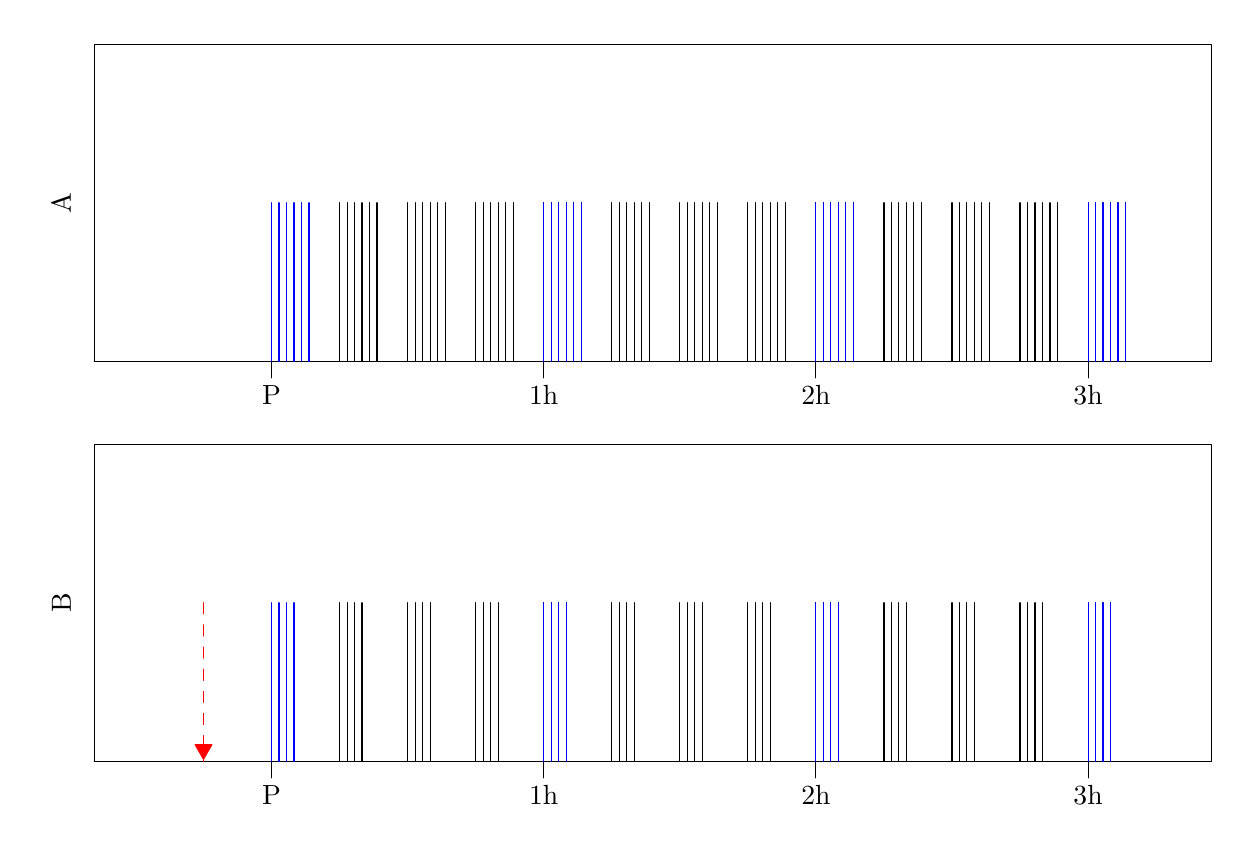
\begin{tikzpicture}[x=1pt,y=1pt]
\definecolor[named]{fillColor}{rgb}{1.00,1.00,1.00}
\path[use as bounding box,fill=fillColor,fill opacity=0.00] (0,0) rectangle (433.62,289.08);
\begin{scope}
\path[clip] (  0.00,  0.00) rectangle (433.62,289.08);
\definecolor[named]{drawColor}{rgb}{0.00,0.00,0.00}

\path[draw=drawColor,line width= 0.4pt,line join=round,line cap=round] ( 24.00,168.54) --
	(427.62,168.54) --
	(427.62,283.08) --
	( 24.00,283.08) --
	( 24.00,168.54);
\end{scope}
\begin{scope}
\path[clip] (  0.00,144.54) rectangle (433.62,289.08);
\definecolor[named]{drawColor}{rgb}{0.00,0.00,0.00}

\node[text=drawColor,rotate= 90.00,anchor=base,inner sep=0pt, outer sep=0pt, scale=  1.00] at ( 15.60,225.81) {A};
\end{scope}
\begin{scope}
\path[clip] (  0.00,  0.00) rectangle (433.62,289.08);
\definecolor[named]{drawColor}{rgb}{0.00,0.00,0.00}

\path[draw=drawColor,line width= 0.4pt,line join=round,line cap=round] ( 88.12,168.54) -- (383.17,168.54);

\path[draw=drawColor,line width= 0.4pt,line join=round,line cap=round] ( 88.12,168.54) -- ( 88.12,162.54);

\path[draw=drawColor,line width= 0.4pt,line join=round,line cap=round] (186.47,168.54) -- (186.47,162.54);

\path[draw=drawColor,line width= 0.4pt,line join=round,line cap=round] (284.82,168.54) -- (284.82,162.54);

\path[draw=drawColor,line width= 0.4pt,line join=round,line cap=round] (383.17,168.54) -- (383.17,162.54);

\node[text=drawColor,anchor=base,inner sep=0pt, outer sep=0pt, scale=  1.00] at ( 88.12,152.94) {P};

\node[text=drawColor,anchor=base,inner sep=0pt, outer sep=0pt, scale=  1.00] at (186.47,152.94) {1h};

\node[text=drawColor,anchor=base,inner sep=0pt, outer sep=0pt, scale=  1.00] at (284.82,152.94) {2h};

\node[text=drawColor,anchor=base,inner sep=0pt, outer sep=0pt, scale=  1.00] at (383.17,152.94) {3h};
\end{scope}
\begin{scope}
\path[clip] ( 24.00,168.54) rectangle (427.62,283.08);
\definecolor[named]{drawColor}{rgb}{0.00,0.00,1.00}

\path[draw=drawColor,line width= 0.4pt,line join=round,line cap=round] ( 88.12, 66.73) -- ( 88.12,225.81);

\path[draw=drawColor,line width= 0.4pt,line join=round,line cap=round] ( 90.83, 66.73) -- ( 90.83,225.81);

\path[draw=drawColor,line width= 0.4pt,line join=round,line cap=round] ( 93.53, 66.73) -- ( 93.53,225.81);

\path[draw=drawColor,line width= 0.4pt,line join=round,line cap=round] ( 96.24, 66.73) -- ( 96.24,225.81);

\path[draw=drawColor,line width= 0.4pt,line join=round,line cap=round] ( 98.94, 66.73) -- ( 98.94,225.81);

\path[draw=drawColor,line width= 0.4pt,line join=round,line cap=round] (101.65, 66.73) -- (101.65,225.81);
\definecolor[named]{drawColor}{rgb}{0.00,0.00,0.00}

\path[draw=drawColor,line width= 0.4pt,line join=round,line cap=round] (112.71, 66.73) -- (112.71,225.81);

\path[draw=drawColor,line width= 0.4pt,line join=round,line cap=round] (115.41, 66.73) -- (115.41,225.81);

\path[draw=drawColor,line width= 0.4pt,line join=round,line cap=round] (118.12, 66.73) -- (118.12,225.81);

\path[draw=drawColor,line width= 0.4pt,line join=round,line cap=round] (120.82, 66.73) -- (120.82,225.81);

\path[draw=drawColor,line width= 0.4pt,line join=round,line cap=round] (123.53, 66.73) -- (123.53,225.81);

\path[draw=drawColor,line width= 0.4pt,line join=round,line cap=round] (126.23, 66.73) -- (126.23,225.81);

\path[draw=drawColor,line width= 0.4pt,line join=round,line cap=round] (137.30, 66.73) -- (137.30,225.81);

\path[draw=drawColor,line width= 0.4pt,line join=round,line cap=round] (140.00, 66.73) -- (140.00,225.81);

\path[draw=drawColor,line width= 0.4pt,line join=round,line cap=round] (142.71, 66.73) -- (142.71,225.81);

\path[draw=drawColor,line width= 0.4pt,line join=round,line cap=round] (145.41, 66.73) -- (145.41,225.81);

\path[draw=drawColor,line width= 0.4pt,line join=round,line cap=round] (148.12, 66.73) -- (148.12,225.81);

\path[draw=drawColor,line width= 0.4pt,line join=round,line cap=round] (150.82, 66.73) -- (150.82,225.81);

\path[draw=drawColor,line width= 0.4pt,line join=round,line cap=round] (161.88, 66.73) -- (161.88,225.81);

\path[draw=drawColor,line width= 0.4pt,line join=round,line cap=round] (164.59, 66.73) -- (164.59,225.81);

\path[draw=drawColor,line width= 0.4pt,line join=round,line cap=round] (167.29, 66.73) -- (167.29,225.81);

\path[draw=drawColor,line width= 0.4pt,line join=round,line cap=round] (170.00, 66.73) -- (170.00,225.81);

\path[draw=drawColor,line width= 0.4pt,line join=round,line cap=round] (172.70, 66.73) -- (172.70,225.81);

\path[draw=drawColor,line width= 0.4pt,line join=round,line cap=round] (175.41, 66.73) -- (175.41,225.81);

\path[draw=drawColor,line width= 0.4pt,line join=round,line cap=round] (186.47, 66.73) -- (186.47,225.81);

\path[draw=drawColor,line width= 0.4pt,line join=round,line cap=round] (189.18, 66.73) -- (189.18,225.81);

\path[draw=drawColor,line width= 0.4pt,line join=round,line cap=round] (191.88, 66.73) -- (191.88,225.81);

\path[draw=drawColor,line width= 0.4pt,line join=round,line cap=round] (194.58, 66.73) -- (194.58,225.81);

\path[draw=drawColor,line width= 0.4pt,line join=round,line cap=round] (197.29, 66.73) -- (197.29,225.81);

\path[draw=drawColor,line width= 0.4pt,line join=round,line cap=round] (199.99, 66.73) -- (199.99,225.81);
\definecolor[named]{drawColor}{rgb}{0.00,0.00,1.00}

\path[draw=drawColor,line width= 0.4pt,line join=round,line cap=round] (186.47, 66.73) -- (186.47,225.81);

\path[draw=drawColor,line width= 0.4pt,line join=round,line cap=round] (189.18, 66.73) -- (189.18,225.81);

\path[draw=drawColor,line width= 0.4pt,line join=round,line cap=round] (191.88, 66.73) -- (191.88,225.81);

\path[draw=drawColor,line width= 0.4pt,line join=round,line cap=round] (194.58, 66.73) -- (194.58,225.81);

\path[draw=drawColor,line width= 0.4pt,line join=round,line cap=round] (197.29, 66.73) -- (197.29,225.81);

\path[draw=drawColor,line width= 0.4pt,line join=round,line cap=round] (199.99, 66.73) -- (199.99,225.81);
\definecolor[named]{drawColor}{rgb}{0.00,0.00,0.00}

\path[draw=drawColor,line width= 0.4pt,line join=round,line cap=round] (211.06, 66.73) -- (211.06,225.81);

\path[draw=drawColor,line width= 0.4pt,line join=round,line cap=round] (213.76, 66.73) -- (213.76,225.81);

\path[draw=drawColor,line width= 0.4pt,line join=round,line cap=round] (216.47, 66.73) -- (216.47,225.81);

\path[draw=drawColor,line width= 0.4pt,line join=round,line cap=round] (219.17, 66.73) -- (219.17,225.81);

\path[draw=drawColor,line width= 0.4pt,line join=round,line cap=round] (221.88, 66.73) -- (221.88,225.81);

\path[draw=drawColor,line width= 0.4pt,line join=round,line cap=round] (224.58, 66.73) -- (224.58,225.81);

\path[draw=drawColor,line width= 0.4pt,line join=round,line cap=round] (235.64, 66.73) -- (235.64,225.81);

\path[draw=drawColor,line width= 0.4pt,line join=round,line cap=round] (238.35, 66.73) -- (238.35,225.81);

\path[draw=drawColor,line width= 0.4pt,line join=round,line cap=round] (241.05, 66.73) -- (241.05,225.81);

\path[draw=drawColor,line width= 0.4pt,line join=round,line cap=round] (243.76, 66.73) -- (243.76,225.81);

\path[draw=drawColor,line width= 0.4pt,line join=round,line cap=round] (246.46, 66.73) -- (246.46,225.81);

\path[draw=drawColor,line width= 0.4pt,line join=round,line cap=round] (249.17, 66.73) -- (249.17,225.81);

\path[draw=drawColor,line width= 0.4pt,line join=round,line cap=round] (260.23, 66.73) -- (260.23,225.81);

\path[draw=drawColor,line width= 0.4pt,line join=round,line cap=round] (262.94, 66.73) -- (262.94,225.81);

\path[draw=drawColor,line width= 0.4pt,line join=round,line cap=round] (265.64, 66.73) -- (265.64,225.81);

\path[draw=drawColor,line width= 0.4pt,line join=round,line cap=round] (268.35, 66.73) -- (268.35,225.81);

\path[draw=drawColor,line width= 0.4pt,line join=round,line cap=round] (271.05, 66.73) -- (271.05,225.81);

\path[draw=drawColor,line width= 0.4pt,line join=round,line cap=round] (273.75, 66.73) -- (273.75,225.81);

\path[draw=drawColor,line width= 0.4pt,line join=round,line cap=round] (284.82, 66.73) -- (284.82,225.81);

\path[draw=drawColor,line width= 0.4pt,line join=round,line cap=round] (287.52, 66.73) -- (287.52,225.81);

\path[draw=drawColor,line width= 0.4pt,line join=round,line cap=round] (290.23, 66.73) -- (290.23,225.81);

\path[draw=drawColor,line width= 0.4pt,line join=round,line cap=round] (292.93, 66.73) -- (292.93,225.81);

\path[draw=drawColor,line width= 0.4pt,line join=round,line cap=round] (295.64, 66.73) -- (295.64,225.81);

\path[draw=drawColor,line width= 0.4pt,line join=round,line cap=round] (298.34, 66.73) -- (298.34,225.81);
\definecolor[named]{drawColor}{rgb}{0.00,0.00,1.00}

\path[draw=drawColor,line width= 0.4pt,line join=round,line cap=round] (284.82, 66.73) -- (284.82,225.81);

\path[draw=drawColor,line width= 0.4pt,line join=round,line cap=round] (287.52, 66.73) -- (287.52,225.81);

\path[draw=drawColor,line width= 0.4pt,line join=round,line cap=round] (290.23, 66.73) -- (290.23,225.81);

\path[draw=drawColor,line width= 0.4pt,line join=round,line cap=round] (292.93, 66.73) -- (292.93,225.81);

\path[draw=drawColor,line width= 0.4pt,line join=round,line cap=round] (295.64, 66.73) -- (295.64,225.81);

\path[draw=drawColor,line width= 0.4pt,line join=round,line cap=round] (298.34, 66.73) -- (298.34,225.81);
\definecolor[named]{drawColor}{rgb}{0.00,0.00,0.00}

\path[draw=drawColor,line width= 0.4pt,line join=round,line cap=round] (309.41, 66.73) -- (309.41,225.81);

\path[draw=drawColor,line width= 0.4pt,line join=round,line cap=round] (312.11, 66.73) -- (312.11,225.81);

\path[draw=drawColor,line width= 0.4pt,line join=round,line cap=round] (314.81, 66.73) -- (314.81,225.81);

\path[draw=drawColor,line width= 0.4pt,line join=round,line cap=round] (317.52, 66.73) -- (317.52,225.81);

\path[draw=drawColor,line width= 0.4pt,line join=round,line cap=round] (320.22, 66.73) -- (320.22,225.81);

\path[draw=drawColor,line width= 0.4pt,line join=round,line cap=round] (322.93, 66.73) -- (322.93,225.81);

\path[draw=drawColor,line width= 0.4pt,line join=round,line cap=round] (333.99, 66.73) -- (333.99,225.81);

\path[draw=drawColor,line width= 0.4pt,line join=round,line cap=round] (336.70, 66.73) -- (336.70,225.81);

\path[draw=drawColor,line width= 0.4pt,line join=round,line cap=round] (339.40, 66.73) -- (339.40,225.81);

\path[draw=drawColor,line width= 0.4pt,line join=round,line cap=round] (342.11, 66.73) -- (342.11,225.81);

\path[draw=drawColor,line width= 0.4pt,line join=round,line cap=round] (344.81, 66.73) -- (344.81,225.81);

\path[draw=drawColor,line width= 0.4pt,line join=round,line cap=round] (347.52, 66.73) -- (347.52,225.81);

\path[draw=drawColor,line width= 0.4pt,line join=round,line cap=round] (358.58, 66.73) -- (358.58,225.81);

\path[draw=drawColor,line width= 0.4pt,line join=round,line cap=round] (361.28, 66.73) -- (361.28,225.81);

\path[draw=drawColor,line width= 0.4pt,line join=round,line cap=round] (363.99, 66.73) -- (363.99,225.81);

\path[draw=drawColor,line width= 0.4pt,line join=round,line cap=round] (366.69, 66.73) -- (366.69,225.81);

\path[draw=drawColor,line width= 0.4pt,line join=round,line cap=round] (369.40, 66.73) -- (369.40,225.81);

\path[draw=drawColor,line width= 0.4pt,line join=round,line cap=round] (372.10, 66.73) -- (372.10,225.81);

\path[draw=drawColor,line width= 0.4pt,line join=round,line cap=round] (383.17, 66.73) -- (383.17,225.81);

\path[draw=drawColor,line width= 0.4pt,line join=round,line cap=round] (385.87, 66.73) -- (385.87,225.81);

\path[draw=drawColor,line width= 0.4pt,line join=round,line cap=round] (388.58, 66.73) -- (388.58,225.81);

\path[draw=drawColor,line width= 0.4pt,line join=round,line cap=round] (391.28, 66.73) -- (391.28,225.81);

\path[draw=drawColor,line width= 0.4pt,line join=round,line cap=round] (393.99, 66.73) -- (393.99,225.81);

\path[draw=drawColor,line width= 0.4pt,line join=round,line cap=round] (396.69, 66.73) -- (396.69,225.81);
\definecolor[named]{drawColor}{rgb}{0.00,0.00,1.00}

\path[draw=drawColor,line width= 0.4pt,line join=round,line cap=round] (383.17, 66.73) -- (383.17,225.81);

\path[draw=drawColor,line width= 0.4pt,line join=round,line cap=round] (385.87, 66.73) -- (385.87,225.81);

\path[draw=drawColor,line width= 0.4pt,line join=round,line cap=round] (388.58, 66.73) -- (388.58,225.81);

\path[draw=drawColor,line width= 0.4pt,line join=round,line cap=round] (391.28, 66.73) -- (391.28,225.81);

\path[draw=drawColor,line width= 0.4pt,line join=round,line cap=round] (393.99, 66.73) -- (393.99,225.81);

\path[draw=drawColor,line width= 0.4pt,line join=round,line cap=round] (396.69, 66.73) -- (396.69,225.81);
\end{scope}
\begin{scope}
\path[clip] (  0.00,  0.00) rectangle (433.62,289.08);
\definecolor[named]{drawColor}{rgb}{0.00,0.00,0.00}

\path[draw=drawColor,line width= 0.4pt,line join=round,line cap=round] ( 24.00, 24.00) --
	(427.62, 24.00) --
	(427.62,138.54) --
	( 24.00,138.54) --
	( 24.00, 24.00);
\end{scope}
\begin{scope}
\path[clip] (  0.00,  0.00) rectangle (433.62,144.54);
\definecolor[named]{drawColor}{rgb}{0.00,0.00,0.00}

\node[text=drawColor,rotate= 90.00,anchor=base,inner sep=0pt, outer sep=0pt, scale=  1.00] at ( 15.60, 81.27) {B};
\end{scope}
\begin{scope}
\path[clip] (  0.00,  0.00) rectangle (433.62,289.08);
\definecolor[named]{drawColor}{rgb}{0.00,0.00,0.00}

\path[draw=drawColor,line width= 0.4pt,line join=round,line cap=round] ( 88.12, 24.00) -- (383.17, 24.00);

\path[draw=drawColor,line width= 0.4pt,line join=round,line cap=round] ( 88.12, 24.00) -- ( 88.12, 18.00);

\path[draw=drawColor,line width= 0.4pt,line join=round,line cap=round] (186.47, 24.00) -- (186.47, 18.00);

\path[draw=drawColor,line width= 0.4pt,line join=round,line cap=round] (284.82, 24.00) -- (284.82, 18.00);

\path[draw=drawColor,line width= 0.4pt,line join=round,line cap=round] (383.17, 24.00) -- (383.17, 18.00);

\node[text=drawColor,anchor=base,inner sep=0pt, outer sep=0pt, scale=  1.00] at ( 88.12,  8.40) {P};

\node[text=drawColor,anchor=base,inner sep=0pt, outer sep=0pt, scale=  1.00] at (186.47,  8.40) {1h};

\node[text=drawColor,anchor=base,inner sep=0pt, outer sep=0pt, scale=  1.00] at (284.82,  8.40) {2h};

\node[text=drawColor,anchor=base,inner sep=0pt, outer sep=0pt, scale=  1.00] at (383.17,  8.40) {3h};
\end{scope}
\begin{scope}
\path[clip] ( 24.00, 24.00) rectangle (427.62,138.54);
\definecolor[named]{drawColor}{rgb}{0.00,0.00,1.00}

\path[draw=drawColor,line width= 0.4pt,line join=round,line cap=round] ( 88.12,  0.00) -- ( 88.12, 81.27);

\path[draw=drawColor,line width= 0.4pt,line join=round,line cap=round] ( 90.83,  0.00) -- ( 90.83, 81.27);

\path[draw=drawColor,line width= 0.4pt,line join=round,line cap=round] ( 93.53,  0.00) -- ( 93.53, 81.27);

\path[draw=drawColor,line width= 0.4pt,line join=round,line cap=round] ( 96.24,  0.00) -- ( 96.24, 81.27);
\definecolor[named]{drawColor}{rgb}{0.00,0.00,0.00}

\path[draw=drawColor,line width= 0.4pt,line join=round,line cap=round] (112.71,  0.00) -- (112.71, 81.27);

\path[draw=drawColor,line width= 0.4pt,line join=round,line cap=round] (115.41,  0.00) -- (115.41, 81.27);

\path[draw=drawColor,line width= 0.4pt,line join=round,line cap=round] (118.12,  0.00) -- (118.12, 81.27);

\path[draw=drawColor,line width= 0.4pt,line join=round,line cap=round] (120.82,  0.00) -- (120.82, 81.27);

\path[draw=drawColor,line width= 0.4pt,line join=round,line cap=round] (137.30,  0.00) -- (137.30, 81.27);

\path[draw=drawColor,line width= 0.4pt,line join=round,line cap=round] (140.00,  0.00) -- (140.00, 81.27);

\path[draw=drawColor,line width= 0.4pt,line join=round,line cap=round] (142.71,  0.00) -- (142.71, 81.27);

\path[draw=drawColor,line width= 0.4pt,line join=round,line cap=round] (145.41,  0.00) -- (145.41, 81.27);

\path[draw=drawColor,line width= 0.4pt,line join=round,line cap=round] (161.88,  0.00) -- (161.88, 81.27);

\path[draw=drawColor,line width= 0.4pt,line join=round,line cap=round] (164.59,  0.00) -- (164.59, 81.27);

\path[draw=drawColor,line width= 0.4pt,line join=round,line cap=round] (167.29,  0.00) -- (167.29, 81.27);

\path[draw=drawColor,line width= 0.4pt,line join=round,line cap=round] (170.00,  0.00) -- (170.00, 81.27);

\path[draw=drawColor,line width= 0.4pt,line join=round,line cap=round] (186.47,  0.00) -- (186.47, 81.27);

\path[draw=drawColor,line width= 0.4pt,line join=round,line cap=round] (189.18,  0.00) -- (189.18, 81.27);

\path[draw=drawColor,line width= 0.4pt,line join=round,line cap=round] (191.88,  0.00) -- (191.88, 81.27);

\path[draw=drawColor,line width= 0.4pt,line join=round,line cap=round] (194.58,  0.00) -- (194.58, 81.27);
\definecolor[named]{drawColor}{rgb}{0.00,0.00,1.00}

\path[draw=drawColor,line width= 0.4pt,line join=round,line cap=round] (186.47,  0.00) -- (186.47, 81.27);

\path[draw=drawColor,line width= 0.4pt,line join=round,line cap=round] (189.18,  0.00) -- (189.18, 81.27);

\path[draw=drawColor,line width= 0.4pt,line join=round,line cap=round] (191.88,  0.00) -- (191.88, 81.27);

\path[draw=drawColor,line width= 0.4pt,line join=round,line cap=round] (194.58,  0.00) -- (194.58, 81.27);
\definecolor[named]{drawColor}{rgb}{0.00,0.00,0.00}

\path[draw=drawColor,line width= 0.4pt,line join=round,line cap=round] (211.06,  0.00) -- (211.06, 81.27);

\path[draw=drawColor,line width= 0.4pt,line join=round,line cap=round] (213.76,  0.00) -- (213.76, 81.27);

\path[draw=drawColor,line width= 0.4pt,line join=round,line cap=round] (216.47,  0.00) -- (216.47, 81.27);

\path[draw=drawColor,line width= 0.4pt,line join=round,line cap=round] (219.17,  0.00) -- (219.17, 81.27);

\path[draw=drawColor,line width= 0.4pt,line join=round,line cap=round] (235.64,  0.00) -- (235.64, 81.27);

\path[draw=drawColor,line width= 0.4pt,line join=round,line cap=round] (238.35,  0.00) -- (238.35, 81.27);

\path[draw=drawColor,line width= 0.4pt,line join=round,line cap=round] (241.05,  0.00) -- (241.05, 81.27);

\path[draw=drawColor,line width= 0.4pt,line join=round,line cap=round] (243.76,  0.00) -- (243.76, 81.27);

\path[draw=drawColor,line width= 0.4pt,line join=round,line cap=round] (260.23,  0.00) -- (260.23, 81.27);

\path[draw=drawColor,line width= 0.4pt,line join=round,line cap=round] (262.94,  0.00) -- (262.94, 81.27);

\path[draw=drawColor,line width= 0.4pt,line join=round,line cap=round] (265.64,  0.00) -- (265.64, 81.27);

\path[draw=drawColor,line width= 0.4pt,line join=round,line cap=round] (268.35,  0.00) -- (268.35, 81.27);

\path[draw=drawColor,line width= 0.4pt,line join=round,line cap=round] (284.82,  0.00) -- (284.82, 81.27);

\path[draw=drawColor,line width= 0.4pt,line join=round,line cap=round] (287.52,  0.00) -- (287.52, 81.27);

\path[draw=drawColor,line width= 0.4pt,line join=round,line cap=round] (290.23,  0.00) -- (290.23, 81.27);

\path[draw=drawColor,line width= 0.4pt,line join=round,line cap=round] (292.93,  0.00) -- (292.93, 81.27);
\definecolor[named]{drawColor}{rgb}{0.00,0.00,1.00}

\path[draw=drawColor,line width= 0.4pt,line join=round,line cap=round] (284.82,  0.00) -- (284.82, 81.27);

\path[draw=drawColor,line width= 0.4pt,line join=round,line cap=round] (287.52,  0.00) -- (287.52, 81.27);

\path[draw=drawColor,line width= 0.4pt,line join=round,line cap=round] (290.23,  0.00) -- (290.23, 81.27);

\path[draw=drawColor,line width= 0.4pt,line join=round,line cap=round] (292.93,  0.00) -- (292.93, 81.27);
\definecolor[named]{drawColor}{rgb}{0.00,0.00,0.00}

\path[draw=drawColor,line width= 0.4pt,line join=round,line cap=round] (309.41,  0.00) -- (309.41, 81.27);

\path[draw=drawColor,line width= 0.4pt,line join=round,line cap=round] (312.11,  0.00) -- (312.11, 81.27);

\path[draw=drawColor,line width= 0.4pt,line join=round,line cap=round] (314.81,  0.00) -- (314.81, 81.27);

\path[draw=drawColor,line width= 0.4pt,line join=round,line cap=round] (317.52,  0.00) -- (317.52, 81.27);

\path[draw=drawColor,line width= 0.4pt,line join=round,line cap=round] (333.99,  0.00) -- (333.99, 81.27);

\path[draw=drawColor,line width= 0.4pt,line join=round,line cap=round] (336.70,  0.00) -- (336.70, 81.27);

\path[draw=drawColor,line width= 0.4pt,line join=round,line cap=round] (339.40,  0.00) -- (339.40, 81.27);

\path[draw=drawColor,line width= 0.4pt,line join=round,line cap=round] (342.11,  0.00) -- (342.11, 81.27);

\path[draw=drawColor,line width= 0.4pt,line join=round,line cap=round] (358.58,  0.00) -- (358.58, 81.27);

\path[draw=drawColor,line width= 0.4pt,line join=round,line cap=round] (361.28,  0.00) -- (361.28, 81.27);

\path[draw=drawColor,line width= 0.4pt,line join=round,line cap=round] (363.99,  0.00) -- (363.99, 81.27);

\path[draw=drawColor,line width= 0.4pt,line join=round,line cap=round] (366.69,  0.00) -- (366.69, 81.27);

\path[draw=drawColor,line width= 0.4pt,line join=round,line cap=round] (383.17,  0.00) -- (383.17, 81.27);

\path[draw=drawColor,line width= 0.4pt,line join=round,line cap=round] (385.87,  0.00) -- (385.87, 81.27);

\path[draw=drawColor,line width= 0.4pt,line join=round,line cap=round] (388.58,  0.00) -- (388.58, 81.27);

\path[draw=drawColor,line width= 0.4pt,line join=round,line cap=round] (391.28,  0.00) -- (391.28, 81.27);
\definecolor[named]{drawColor}{rgb}{0.00,0.00,1.00}

\path[draw=drawColor,line width= 0.4pt,line join=round,line cap=round] (383.17,  0.00) -- (383.17, 81.27);

\path[draw=drawColor,line width= 0.4pt,line join=round,line cap=round] (385.87,  0.00) -- (385.87, 81.27);

\path[draw=drawColor,line width= 0.4pt,line join=round,line cap=round] (388.58,  0.00) -- (388.58, 81.27);

\path[draw=drawColor,line width= 0.4pt,line join=round,line cap=round] (391.28,  0.00) -- (391.28, 81.27);
\definecolor[named]{drawColor}{rgb}{1.00,0.00,0.00}

\path[draw=drawColor,line width= 0.4pt,dash pattern=on 4pt off 4pt ,line join=round,line cap=round] ( 63.54, 81.27) -- ( 63.54,  0.00);
\definecolor[named]{fillColor}{rgb}{1.00,0.00,0.00}

\path[draw=drawColor,line width= 0.4pt,line join=round,line cap=round,fill=fillColor] ( 63.54, 24.74) --
	( 66.57, 29.99) --
	( 60.51, 29.99) --
	cycle;
\end{scope}
\end{tikzpicture}
